\documentclass[a4paper]{article}

\def\npart {II}
\def\nterm {Michaelmas}
\def\nyear {2016}
\def\nlecturer {A. Ashton}
\def\ncourse {Integrable Systems}
\def\nlectures {TT.11}

% Imports
\ifx \nextra \undefined
  \usepackage[pdftex,
    hidelinks,
    pdfauthor={Dexter Chua},
    pdfsubject={Cambridge Maths Notes: Part \npart\ - \ncourse},
    pdftitle={Part \npart\ - \ncourse},
  pdfkeywords={Cambridge Mathematics Maths Math \npart\ \nterm\ \nyear\ \ncourse}]{hyperref}
  \title{Part \npart\ - \ncourse}
\else
  \usepackage[pdftex,
    hidelinks,
    pdfauthor={Dexter Chua},
    pdfsubject={Cambridge Maths Notes: Part \npart\ - \ncourse\ (\nextra)},
    pdftitle={Part \npart\ - \ncourse\ (\nextra)},
  pdfkeywords={Cambridge Mathematics Maths Math \npart\ \nterm\ \nyear\ \ncourse\ \nextra}]{hyperref}

  \title{Part \npart\ - \ncourse \\ {\Large \nextra}}
\fi

\author{Lectured by \nlecturer \\\small Notes taken by Dexter Chua}
\date{\nterm\ \nyear}

\usepackage{alltt}
\usepackage{amsfonts}
\usepackage{amsmath}
\usepackage{amssymb}
\usepackage{amsthm}
\usepackage{booktabs}
\usepackage{caption}
\usepackage{enumitem}
\usepackage{fancyhdr}
\usepackage{graphicx}
\usepackage{mathtools}
\usepackage{microtype}
\usepackage{multirow}
\usepackage{pdflscape}
\usepackage{pgfplots}
\usepackage{siunitx}
\usepackage{tabularx}
\usepackage{tikz}
\usepackage{tkz-euclide}
\usepackage[normalem]{ulem}
\usepackage[all]{xy}

\pgfplotsset{compat=1.12}

\pagestyle{fancyplain}
\lhead{\emph{\nouppercase{\leftmark}}}
\ifx \nextra \undefined
  \rhead{
    \ifnum\thepage=1
    \else
      \npart\ \ncourse
    \fi}
\else
  \rhead{
    \ifnum\thepage=1
    \else
      \npart\ \ncourse\ (\nextra)
    \fi}
\fi
\usetikzlibrary{arrows}
\usetikzlibrary{decorations.markings}
\usetikzlibrary{decorations.pathmorphing}
\usetikzlibrary{positioning}
\usetikzlibrary{fadings}
\usetikzlibrary{intersections}
\usetikzlibrary{cd}

\newcommand*{\Cdot}{\raisebox{-0.25ex}{\scalebox{1.5}{$\cdot$}}}
\newcommand {\pd}[2][ ]{
  \ifx #1 { }
    \frac{\partial}{\partial #2}
  \else
    \frac{\partial^{#1}}{\partial #2^{#1}}
  \fi
}

% Theorems
\theoremstyle{definition}
\newtheorem*{aim}{Aim}
\newtheorem*{axiom}{Axiom}
\newtheorem*{claim}{Claim}
\newtheorem*{cor}{Corollary}
\newtheorem*{defi}{Definition}
\newtheorem*{eg}{Example}
\newtheorem*{fact}{Fact}
\newtheorem*{law}{Law}
\newtheorem*{lemma}{Lemma}
\newtheorem*{notation}{Notation}
\newtheorem*{prop}{Proposition}
\newtheorem*{thm}{Theorem}

\renewcommand{\labelitemi}{--}
\renewcommand{\labelitemii}{$\circ$}
\renewcommand{\labelenumi}{(\roman{*})}

\let\stdsection\section
\renewcommand\section{\newpage\stdsection}

% Strike through
\def\st{\bgroup \ULdepth=-.55ex \ULset}

% Maths symbols
\newcommand{\bra}{\langle}
\newcommand{\ket}{\rangle}

\newcommand{\N}{\mathbb{N}}
\newcommand{\Z}{\mathbb{Z}}
\newcommand{\Q}{\mathbb{Q}}
\renewcommand{\H}{\mathbb{H}}
\newcommand{\R}{\mathbb{R}}
\newcommand{\C}{\mathbb{C}}
\newcommand{\Prob}{\mathbb{P}}
\renewcommand{\P}{\mathbb{P}}
\newcommand{\E}{\mathbb{E}}
\newcommand{\F}{\mathbb{F}}
\newcommand{\cU}{\mathcal{U}}
\newcommand{\RP}{\mathbb{RP}}
\newcommand{\CP}{\mathbb{CP}}

\newcommand{\ph}{\,\cdot\,}

\DeclareMathOperator{\sech}{sech}
\DeclareMathOperator{\cosech}{cosech}
\DeclareMathOperator{\cosec}{cosec}

\DeclareMathOperator{\covol}{covol}
\DeclareMathOperator{\vol}{vol}

\let\Im\relax
\let\Re\relax
\DeclareMathOperator{\Im}{Im}
\DeclareMathOperator{\Re}{Re}
\DeclareMathOperator{\im}{im}
\DeclareMathOperator{\image}{image}
\DeclareMathOperator{\Ann}{Ann}

\DeclareMathOperator*{\res}{res}
\DeclareMathOperator{\Res}{Res}
\DeclareMathOperator{\Ind}{Ind}

\DeclareMathOperator{\tr}{tr}
\DeclareMathOperator{\diag}{diag}
\DeclareMathOperator{\rank}{rank}
\DeclareMathOperator{\card}{card}
\DeclareMathOperator{\spn}{span}
\DeclareMathOperator{\adj}{adj}

\DeclareMathOperator{\erf}{erf}
\DeclareMathOperator{\erfc}{erfc}

\DeclareMathOperator{\ord}{ord}
\DeclareMathOperator{\Sym}{Sym}

\DeclareMathOperator{\sgn}{sgn}
\DeclareMathOperator{\orb}{orb}
\DeclareMathOperator{\stab}{stab}
\DeclareMathOperator{\ccl}{ccl}

\DeclareMathOperator{\lcm}{lcm}
\DeclareMathOperator{\hcf}{hcf}

\DeclareMathOperator{\Int}{Int}
\DeclareMathOperator{\id}{id}

\DeclareMathOperator{\betaD}{beta}
\DeclareMathOperator{\gammaD}{gamma}
\DeclareMathOperator{\Poisson}{Poisson}
\DeclareMathOperator{\binomial}{binomial}
\DeclareMathOperator{\multinomial}{multinomial}
\DeclareMathOperator{\Bernoulli}{Bernoulli}
\DeclareMathOperator{\like}{like}

\DeclareMathOperator{\var}{var}
\DeclareMathOperator{\cov}{cov}
\DeclareMathOperator{\bias}{bias}
\DeclareMathOperator{\mse}{mse}
\DeclareMathOperator{\corr}{corr}

\DeclareMathOperator{\otp}{otp}
\DeclareMathOperator{\dom}{dom}

\DeclareMathOperator{\Root}{Root}
\DeclareMathOperator{\supp}{supp}
\DeclareMathOperator{\rel}{rel}
\DeclareMathOperator{\Hom}{Hom}
\DeclareMathOperator{\Aut}{Aut}
\DeclareMathOperator{\Gal}{Gal}
\DeclareMathOperator{\Mat}{Mat}
\DeclareMathOperator{\End}{End}
\DeclareMathOperator{\Char}{char}
\DeclareMathOperator{\ev}{ev}
\DeclareMathOperator{\St}{St}
\DeclareMathOperator{\Lk}{Lk}
\DeclareMathOperator{\disc}{disc}
\DeclareMathOperator{\Isom}{Isom}
\DeclareMathOperator{\length}{length}
\DeclareMathOperator{\energy}{energy}
\DeclareMathOperator{\area}{area}
\DeclareMathOperator{\Syl}{Syl}
\DeclareMathOperator{\cl}{cl}
\DeclareMathOperator{\fix}{fix}

\newcommand{\GL}{\mathrm{GL}}
\newcommand{\SL}{\mathrm{SL}}
\newcommand{\PGL}{\mathrm{PGL}}
\newcommand{\PSL}{\mathrm{PSL}}
\newcommand{\PSU}{\mathrm{PSU}}
\newcommand{\Or}{\mathrm{O}}
\newcommand{\SO}{\mathrm{SO}}
\newcommand{\U}{\mathrm{U}}
\newcommand{\SU}{\mathrm{SU}}

\renewcommand{\d}{\mathrm{d}}
\newcommand{\D}{\mathrm{D}}

\tikzset{->/.style = {decoration={markings,
                                  mark=at position 1 with {\arrow[scale=2]{latex'}}},
                      postaction={decorate}}}
\tikzset{<-/.style = {decoration={markings,
                                  mark=at position 0 with {\arrowreversed[scale=2]{latex'}}},
                      postaction={decorate}}}
\tikzset{<->/.style = {decoration={markings,
                                   mark=at position 0 with {\arrowreversed[scale=2]{latex'}},
                                   mark=at position 1 with {\arrow[scale=2]{latex'}}},
                       postaction={decorate}}}
\tikzset{->-/.style = {decoration={markings,
                                   mark=at position #1 with {\arrow[scale=2]{latex'}}},
                       postaction={decorate}}}
\tikzset{-<-/.style = {decoration={markings,
                                   mark=at position #1 with {\arrowreversed[scale=2]{latex'}}},
                       postaction={decorate}}}

\tikzset{circ/.style = {fill, circle, inner sep = 0, minimum size = 3}}
\tikzset{mstate/.style={circle, draw, blue, text=black, minimum width=0.7cm}}

\definecolor{mblue}{rgb}{0.2, 0.3, 0.8}
\definecolor{morange}{rgb}{1, 0.5, 0}
\definecolor{mgreen}{rgb}{0.1, 0.4, 0.2}
\definecolor{mred}{rgb}{0.5, 0, 0}

\def\drawcirculararc(#1,#2)(#3,#4)(#5,#6){%
    \pgfmathsetmacro\cA{(#1*#1+#2*#2-#3*#3-#4*#4)/2}%
    \pgfmathsetmacro\cB{(#1*#1+#2*#2-#5*#5-#6*#6)/2}%
    \pgfmathsetmacro\cy{(\cB*(#1-#3)-\cA*(#1-#5))/%
                        ((#2-#6)*(#1-#3)-(#2-#4)*(#1-#5))}%
    \pgfmathsetmacro\cx{(\cA-\cy*(#2-#4))/(#1-#3)}%
    \pgfmathsetmacro\cr{sqrt((#1-\cx)*(#1-\cx)+(#2-\cy)*(#2-\cy))}%
    \pgfmathsetmacro\cA{atan2(#2-\cy,#1-\cx)}%
    \pgfmathsetmacro\cB{atan2(#6-\cy,#5-\cx)}%
    \pgfmathparse{\cB<\cA}%
    \ifnum\pgfmathresult=1
        \pgfmathsetmacro\cB{\cB+360}%
    \fi
    \draw (#1,#2) arc (\cA:\cB:\cr);%
}
\newcommand\getCoord[3]{\newdimen{#1}\newdimen{#2}\pgfextractx{#1}{\pgfpointanchor{#3}{center}}\pgfextracty{#2}{\pgfpointanchor{#3}{center}}}

\def\Xint#1{\mathchoice
   {\XXint\displaystyle\textstyle{#1}}%
   {\XXint\textstyle\scriptstyle{#1}}%
   {\XXint\scriptstyle\scriptscriptstyle{#1}}%
   {\XXint\scriptscriptstyle\scriptscriptstyle{#1}}%
   \!\int}
\def\XXint#1#2#3{{\setbox0=\hbox{$#1{#2#3}{\int}$}
     \vcenter{\hbox{$#2#3$}}\kern-.5\wd0}}
\def\ddashint{\Xint=}
\def\dashint{\Xint-}


\begin{document}
\maketitle
{\small
\noindent\emph{Part IB Methods, and Complex Methods or Complex Analysis are essential; Part II Classical Dynamics is desirable.}

\vspace{10pt}
\noindent Integrability of ordinary differential equations: Hamiltonian systems and the Arnol'd--Liouville Theorem (sketch of proof). Examples.\hspace*{\fill}[3]

\vspace{5pt}
\noindent Integrability of partial differential equations: The rich mathematical structure and the universality of the integrable nonlinear partial differential equations (Korteweg-de Vries, sine-Gordon). Backlund transformations and soliton solutions.\hspace*{\fill}[2]

\vspace{5pt}
\noindent The inverse scattering method: Lax pairs. The inverse scattering method for the KdV equation, and other integrable PDEs. Multi soliton solutions. Zero curvature representation. \hspace*{\fill}[6]

\vspace{5pt}
\noindent Hamiltonian formulation of soliton equations.\hspace*{\fill}[2]

\vspace{5pt}
\noindent Painleve equations and Lie symmetries: Symmetries of differential equations, the ODE reductions of certain integrable nonlinear PDEs, Painleve equations.\hspace*{\fill}[3]%
}

\tableofcontents
\setcounter{section}{-1}
\section{Introduction}
What is an integrable system? Unfortunately, an integrable system is a something mathematicians have not yet managed to define properly. Intuitively, an integrable system is a differential equation we can ``integrate up'' directly. While in theory, integrable systems should be very rare, it happens that in nature, a lot of systems happen to be integrable. By exploiting the fact that they are integrable, we can solve them much more easily.

\section{Integrability of ODEs}
\subsection{Vector fields and flow maps}
For a vector field $\mathbf{V}: \R^m \to \R^m$, consider a differential equation for $\mathbf{x}(t) \in \R^m$,
\[
  \dot{\mathbf{x}} = \mathbf{V}(\mathbf{x}),\quad \mathbf{x}(0) = \mathbf{x}_0.
\]
In this course, we will assume the vector field $\mathbf{V}$ is ``nice'', in the sense that the solutions always exist and are unique, and are infinitely differentiable.

It is convenient to write the solution as
\[
  \mathbf{x}(t) = g^t \mathbf{x}_0,
\]
where $g^t: \R^m \to \R^m$ is called the \emph{flow map}. This has some nice properties:
\begin{prop}\leavevmode
  \begin{enumerate}
    \item $g_0 = \id$
    \item $g^{t + s} = g^t g^s$
    \item $(g^{t})^{-1} = g^{-t}$
  \end{enumerate}
\end{prop}
The proofs are left for the first example sheet.

We say that $\mathbf{V}$ is the \emph{infinitesimal generator} of the flow $g^t$. This is because
\[
  \mathbf{x}(\varepsilon) = g^\varepsilon \mathbf{x}_0 = \mathbf{x}(0) + \varepsilon \dot{\mathbf{x}}(0) + o(\varepsilon) = \mathbf{x}_0 + \varepsilon \mathbf{V}(\mathbf{x}_0) + o(\varepsilon).
\]
For two vector fields $\mathbf{V}_1, \mathbf{V}_2: \R^m \to \R^m$ which generate flows $g_1^t$ and $g_2^s$, we define the third vector field, the commutator, by
\[
  [\mathbf{V}_1, \mathbf{V}_2] = \left(\mathbf{V}_1 \cdot \frac{\partial}{\partial \mathbf{x}}\right) \mathbf{V}_2 - \left(\mathbf{V}_2 \cdot \frac{\partial}{\partial \mathbf{x}}\right) \mathbf{V}_1,
\]
where we write
\[
  \frac{\partial}{\partial \mathbf{x}} = \left(\frac{\partial}{\partial x_1}, \cdots, \frac{\partial}{\partial x_n}\right)^T.
\]
More explicitly, the $i$th component
\[
  [\mathbf{V}_1, \mathbf{V}_2]_i = \sum_{j = 1}^m (\mathbf{v}_1)_j \frac{\partial}{\partial x_j} (\mathbf{v}_2)_i - (\mathbf{v}_2)_j \frac{\partial}{\partial x_j} (\mathbf{v}_1)_i
\]
This is a very important concept, because we have
\begin{prop}
  \[
    [\mathbf{V}_1, \mathbf{V}_2] = 0 \Leftrightarrow g_1^t g_2^s = g_2^s g_1^t.
  \]
\end{prop}
This will be shown in the first example sheet.

Thus, to figure out if two flows commute, it suffices to check if their infinitesimal generates commutative.
\subsection{Phase space and Poisson brackets}
In this section, we are interested in dynamical problems on a $2n$-dimensional \emph{phase space} $M$. Points on $M$ are described by coordinates
\[
  (\mathbf{q}, \mathbf{p}) = (q_1, \cdots, q_n, p_1, \cdots, p_n).
\]
We tend to think of the $q_i$ are ``generalized positions'' of particles, and the $p_n$ as the ``generalized momentum'' coordinates. We will often write
\[
  \mathbf{x} = (\mathbf{q}, \mathbf{p})^T.
\]
We introduce a $2n \times 2n$ anti-symmetric matrix
\[
  J =
  \begin{pmatrix}
    0 & I_n\\
    -I_n & 0
  \end{pmatrix}.
\]
We are now going to define a \emph{Poisson bracket}.

\begin{defi}[Poisson bracket]
  For any two functions $f, g: M \to \R$, we define the \emph{Poisson bracket} by
  \[
    \{f, g\} = \frac{\partial f}{\partial \mathbf{x}} J \frac{\partial g}{\partial \mathbf{x}} = \frac{\partial f}{\partial \mathbf{q}} \cdot \frac{\partial g}{\partial \mathbf{p}} - \frac{\partial f}{\partial \mathbf{p}} \cdot \frac{\partial g}{\partial \mathbf{q}}.
  \]
\end{defi}

This has some obvious and not-so-obvious properties:
\begin{prop}\leavevmode
  \begin{enumerate}
    \item This is linear in each argument.
    \item This is antisymmetric, ie. $\{f, g\} = - \{g, f\}$.
    \item Leibniz property: $\{f, gh\} = \{f, g\}h + \{f, h\} g$.
    \item Jacobi identity: $\{f, \{g, h\}\} + \{g, \{h, f\}\} + \{h, \{f, g\}\} = 0$.
    \item
      \[
        \{q_i, q_j\} = \{p_i, p_j\} = 0,\quad \{q_i, p_j\} = \delta_{ij}.
      \]
  \end{enumerate}
\end{prop}

\subsection{Hamiltonian dynamics}
We will be interested in problems on $M$ of the following form:
\begin{defi}[Hamilton's equation]
  \emph{Hamilton's equation} is an equation of the form
  \[
    \dot{\mathbf{q}} = \frac{\partial H}{\partial \mathbf{p}},\quad \dot{\mathbf{p}} = -\frac{\partial H}{\partial \mathbf{q}}\tag{$*$}
  \]
  For some function $H: M \to \R$ called the \emph{Hamiltonian}.
\end{defi}
Just as we think of $\mathbf{q}$ and $\mathbf{p}$ as generalized position and momentum, we tend to think of $H$ as generalized energy.

Note that $(*)$ can be written as
\[
  \dot{\mathbf{x}} = J \frac{\partial H}{\partial \mathbf{x}}.
\]
Compare this to the equation
\[
  \dot{\mathbf{x}} = \mathbf{V}(\mathbf{x}), \quad \mathbf{x}(0) = \mathbf{x}_0.
\]
Assuming that $\mathbf{x}$ evolves according to Hamilton's equations, if $f: M \to \R$ is a smooth function, then by the chain rule, we have
\begin{align*}
  \frac{\d f}{\d t} &= \frac{\d}{\d t} f(\mathbf{q}(t), \mathbf{p}(t))\\
  &= \frac{\partial f}{\partial \mathbf{q}} \cdot \dot{\mathbf{q}} + \frac{\partial f}{\partial \mathbf{p}} \cdot \dot{\mathbf{p}}\\
  &= \frac{\partial f}{\partial \mathbf{q}} \cdot \frac{\partial H}{\partial \mathbf{p}} - \frac{\partial f}{\partial \mathbf{p}} \cdot \frac{\partial H}{\partial \mathbf{q}} \\
  &= \{f, H\}.
\end{align*}
In particular, we have
\[
  \frac{\d H}{\d t} = \{H, H\} = 0.
\]
So the Hamiltonian is constant!
\begin{eg}
  Consider a particle (of unit mass) with position $\mathbf{q} = (q_1, q_2, q_3)$ (in Cartesian coordinates) moving under the influence of a potential $U(\mathbf{q})$. By Newton's second law, we have
  \[
    \ddot{\mathbf{q}} = -\frac{\partial U}{\partial \mathbf{q}}.
  \]
  This is actually a Hamiltonian system. We define the momentum variables by
  \[
    p_i = \dot{q}_i,
  \]
  then we have
  \[
    \dot{\mathbf{x}} =
    \begin{pmatrix}
      \dot{\mathbf{q}}
      \dot{\mathbf{p}}
    \end{pmatrix}
    =
    \begin{pmatrix}
      \mathbf{p}\\
      -\frac{\partial U}{\partial \mathbf{q}}
    \end{pmatrix}
    = J \frac{\partial H}{\partial \mathbf{x}},
  \]
  with
  \[
    H = \frac{1}{2} |\mathbf{p}|^2 + U(\mathbf{q}).
  \]
  This is just the usual energy! Indeed, we have
  \[
    \frac{\partial H}{\partial \mathbf{p}} = \mathbf{p},\quad \frac{\partial H}{\partial \mathbf{q}} = \frac{\partial H}{\partial \mathbf{q}}.
  \]
\end{eg}

\begin{defi}[Hamiltonian vector field]\index{Hamiltonian vector field}
  Given a Hamiltonian function $H$, the \emph{Hamiltonian vector field} is given by
  \[
    \mathbf{V}_H = J \frac{\partial H}{\partial \mathbf{x}}.
  \]
\end{defi}

We then see that the Hamiltonian vector field generates the Hamiltonian flow. More generally, for any $f: M \to \R$, we call
\[
  \mathbf{V}_f = J \frac{\partial f}{\partial \mathbf{x}}.
\]
This is the Hamiltonian vector field with respect to $f$ and $g$.

\begin{prop}
  We have
  \[
    [V_\mathbf{f}, V_\mathbf{g}] = - \mathbf{V}_{\{f, g\}}.
  \]
\end{prop}

\begin{proof}
  See first example sheet. % Fill in
\end{proof}

\begin{defi}[First integral]\index{first integral}
  Given a phase space $M$ with a Hamiltonian $H$, we call $f: M \to \R$ a \emph{first integral} of the Hamiltonian system if
  \[
    \{f, H\} = 0.
  \]
\end{defi}
The reason for the term ``first integral'' is historical --- when we solve a differential equation, we integrate the equation. Every time we integrate it, we obtain a new constant. And the first constant we obtain when we integrate is known as the first integral. However, for our purposes, we can just as well think of it as a constant of motion.

\begin{eg}
  Consider the two-body problem --- the Sun is fixed at the origin, and a planet has Cartesian coordinates $\mathbf{q} = (q_1, q_2, q_3)$. The equation of motion will be
  \[
    \ddot{\mathbf{q}} = - \frac{\mathbf{q}}{|\mathbf{q}|^3}.
  \]
  This is equivalent to the Hamiltonian system $\mathbf{p} = \dot{\mathbf{q}}$, with
  \[
    H = \frac{1}{2} |\mathbf{p}|^2 - \frac{1}{|\mathbf{q}|}.
  \]
  We have an angular momentum given by
  \[
    \mathbf{L} = \mathbf{q} \wedge \mathbf{p}.
  \]
  Working with coordinates, we have
  \[
    L_i = \varepsilon_{ijk} q_j p_k.
  \]
  We then have
  \begin{align*}
    \{L_i, H\} &= \frac{\partial L_i}{\partial q_\ell}\frac{\partial H}{\partial p_\ell} - \frac{\partial L_i}{\partial p_\ell} \frac{\partial H}{\partial q_\ell}\\
    &= \varepsilon_{ijk} \left(p_k \delta_{\ell j}p_\ell + \frac{q_j q_k}{|\mathbf{q}|^3}\right)\\
    &= \varepsilon_{ijk} \left(p_k p_j + \frac{q_j q_k}{|\mathbf{q}|^3}\right)\\
    &= 0,
  \end{align*}
  where we know the thing vanishes because we contracted a symmetric tensor with an antisymmetric one. So this is a first integral.

  Less interestingly, we know $H$ is also a first integral. In general, some Hamiltonian have many many first integrals.
\end{eg}

\begin{defi}[Involution]\index{involution}
  We say that two first integrals $F, G$ are in \emph{involution} if $\{F, G\} = 0$ (so $F$ and $G$ ``\emph{Poisson commute}'').
\end{defi}

\begin{defi}[Independent first integrals]\index{independent first integrals}
  A collection of functions $f_i: M \to \R$ are independent if at each $\mathbf{x} \in M$, the vectors $\frac{\partial f_i}{\partial \mathbf{x}}$ for $i = 1, \cdots, n$ are independent.
\end{defi}

\begin{defi}[Integrable system]\index{integrable system}
  A $2n$-dimensional Hamiltonian system $(M, H)$ is \emph{integrable} if there exists $n$ first integrals $\{f_i\}_{i = 1}^n$ that are independent and in involution (ie. $\{f_i, f_j\} = 0$ for all $i, j$).
\end{defi}
The word independent is very important, or else people will cheat, eg. take $H, 2H, e^H, H^2, \cdots$.

\begin{cor}
  Two-dimensional Hamiltonian systems are always integrable.
\end{cor}

We are now ready for the main section.
%\section{Action-angle coordinates and the Arnold-Liouville theorem}
\section{The Arnold-Liouville theorem}
Consider the Hamiltonian system
\[
  \dot{\mathbf{q}} = \frac{\partial H}{\partial \mathbf{q}},\quad \mathbf{p} = -\frac{\partial H}{\partial \mathbf{q}}.
\]
We do not expect a general coordinate change $(\mathbf{q}, \mathbf{p}) \mapsto (\mathbf{Q}(\mathbf{q}, \mathbf{q}), \mathbf{P}(\mathbf{q}, \mathbf{p}))$ to hold the form of Hamilton's equations, ie. we will no longer have
\[
  \dot{\mathbf{Q}} = \frac{\partial \tilde{H}}{\partial \mathbf{P}},\quad \dot{\mathbf{P}} = -\frac{\partial \tilde{H}}{\partial \mathbf{Q}},
\]
where $\tilde{H}(\mathbf{Q}, \mathbf{P}) = H(\mathbf{q}, \mathbf{p})$.

If we write $\mathbf{x} = (\mathbf{q}, \mathbf{p})$ and $\mathbf{y} = (\mathbf{Q}, \mathbf{P})$, then this is equivalent to asking if
\[
  \dot{\mathbf{x}} = J \frac{\partial H}{\partial \mathbf{x}} \quad\Rightarrow\quad \dot{\mathbf{y}} = J \frac{\partial \tilde{H}}{ \partial \mathbf{y}}.
\]
For example, if we just swap $\mathbf{p}$ and $\mathbf{q}$ around, the form of the equation changes (namely the signs go in the wrong place).

\begin{defi}[Canonical transformation]\index{canonical transformation}
  A coordinate change $(\mathbf{q}, \mathbf{p}) \mapsto (\mathbf{Q}, \mathbf{P})$ is called \emph{canonical} if it leaves Hamilton's equations invariant, ie. we have
  \[
    \dot{\mathbf{Q}} = \frac{\partial \tilde{H}}{\partial \mathbf{P}},\quad \dot{\mathbf{P}} = -\frac{\partial \tilde{H}}{\partial \mathbf{Q}},
  \]
\end{defi}

\begin{eg}
  The simplest possible case of a canonical transformation is a linear transformation. Consider a linear change of coordinates given by
  \[
    \mathbf{x} \mapsto \mathbf{y}(\mathbf{x}) = A\mathbf{x}.
  \]
  We claim that this is canonical iff $AJA^t = J$, ie. that $A$ is \term{symplectic}.

  Indeed, by linearity, we have
  \[
    \dot{\mathbf{y}} = A\dot{\mathbf{x}} = AJ\frac{\partial H}{\mathbf{x}}.
  \]
  Setting $\tilde{\mathbf{H}}(\mathbf{y} = H(\mathbf{x})$, we have
  \[
    \frac{\partial H}{\partial x_i} = \frac{\partial y_j}{\partial x_i} \frac{\partial \tilde{H}(\mathbf{y})}{\partial y_j} = A_{ji} \frac{\partial \tilde{H}(\mathbf{y})}{\partial y_j}(\mathbf{y}) = \left[A^T \frac{\partial \tilde{H}}{\partial \mathbf{y}}\right]_i.
  \]
  Putting this back in, we have
  \[
    \dot{\mathbf{y}} = AJA^T \frac{\partial\tilde{H}}{\partial \mathbf{y}}.
  \]
  So $\mathbf{y} \mapsto \mathbf{y}(\mathbf{x})$ is canonical if $J = AJA^T$.
\end{eg}

What about more general cases? Recall from IB Analysis II that a map is differentiable if it is ``locally linear''. Now Hamilton's equations are purely local equations, so we might expect the following:
\begin{prop}
  A map $\mathbf{x} \mapsto \mathbf{y}(\mathbf{x})$ is canonical iff $D\mathbf{y}$ is symplectic, ie.
  \[
    D\mathbf{y} J (D\mathbf{y})^T = J.
  \]
\end{prop}

Now could we find a canonical transformation $(\mathbf{q}, \mathbf{p}) \mapsto (\mathbf{Q}, \mathbf{P})$ such that $\tilde{H}$ depends only on $\mathbf{P}$. If this happened, then Hamilton's equations reduce to
\[
  \dot{\mathbf{Q}} = \frac{\partial \tilde{H}}{\partial \mathbf{P}}(\mathbf{P}),\quad \dot{\mathbf{P}} = -\frac{\partial \tilde{H}}{\partial \mathbf{Q}} = 0.
\]
So $\mathbf{P}(t) = \mathbf{P}_0$ is a constant. Since the right hand side of the first equation depends only on $\mathbf{P}$, we find that $\dot{\mathbf{Q}}$ is also constant! So $\mathbf{Q} = \mathbf{Q}_0 + \Omega t$, where
\[
  \Omega = \frac{\partial \tilde{H}}{\partial \mathbf{P}} (\mathbf{P}_0).
\]
So if we could find a good canonical transformation, the solution falls out easily! It turns out that if a system is integrable, then we can indeed find such coordinates.

We are now going to prove the Arnold-Liouville theorem. Before we do that in full generality, we first do it in a specific case, and see how the proof actually works out.

\begin{eg}
  Consider the harmonic oscillator with Hamiltonian
  \[
    H(q, p) = \frac{1}{2}p^2 + \frac{1}{2}\omega^2 q^2.
  \]
  Since is a 2-dimensional system, so we only need a single first integral. Since $H$ is a first integral for trivial reasons, this is an integrable Hamiltonian system.

  We can actually draw the lines on which $H$ is constant --- they are just ellipses:
  \begin{center}
    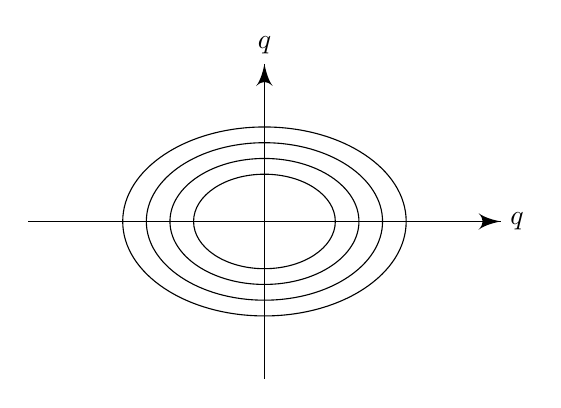
\begin{tikzpicture}
      \draw [->] (-3, 0) -- (3, 0) node [right] {$q$};
      \draw [->] (0, -2) -- (0, 2) node [above] {$q$};

      \foreach \x in {0.6, 0.8, 1, 1.2} {
        \begin{scope}[scale=\x]
          \draw ellipse (1.5 and 1);
        \end{scope}
      }
    \end{tikzpicture}
  \end{center}
  We note that the ellipses are homeomorphic to $S^1$. Now we introduce the coordinate transformation $(q, p) \mapsto (\phi, I)$, defined by
  \[
    q = \sqrt{\frac{2I}{\omega}} \sin \phi,\quad p = \sqrt{2I\omega} \cos \phi,
  \]
  For the purpose of this example, we can suppose we obtained this formula through divine inspiration. However, in the Arnold-Liouville theorem, we will provide a general way of coming up with these formulas.

  We can manually show that this transformation is canonical (it is actually easier to show that the inverse map $(\phi, I) \mapsto (q, p)$ is canonical). We also have that
  \[
    \tilde{H}(\phi, I) = H(q(\phi, I), p(\phi, I)) = \omega I.
  \]
  This is really nice. There is no $\phi$! Now Hamilton's equations become
  \[
    \dot\phi = \frac{\partial \tilde{H}}{ \partial I} = \omega,\quad \dot{I} = -\frac{\partial \tilde{H}}{\partial \phi} = 0.
  \]
  We can integrate up to obtain
  \[
    \phi(t) = \phi_0 + \omega t,\quad I(t) = I_0.
  \]
  It is fun to consider the integral along paths of constant $H$:
  \begin{align*}
    \frac{1}{2\pi}\oint p \;\d q &= \frac{1}{2\pi} \int_0^{2\pi}p(\phi, I) \left(\frac{\partial q}{\partial \phi} \;\d \phi + \frac{\partial q}{\partial I} \;\d I\right)\\
    &= \frac{1}{2\pi} \int_0^{2\pi}p(\phi, I) \left(\frac{\partial q}{\partial \phi} \;\d \phi\right)\\
    &= \frac{1}{2\pi} \int_0^{2\pi} \sqrt{\frac{2I}{\omega}}\sqrt{2I\omega} \cos^2 \phi \;\d \phi\\
    &= I
  \end{align*}
  This is interesting. We didn't know how we obtained $I$, but in fact we can obtain it by performing an integral like this.
\end{eg}
There are two things to take away from this.
\begin{enumerate}
  \item The motion takes place in $S^1$
  \item We got $I$ by performing $\frac{1}{2\pi}\oint p \;\d q$.
\end{enumerate}
These two ideas are essentially what we are going to prove for general Hamiltonian system.

\begin{thm}[Arnold-Liouville theorem]\index{Arnold-Liouville theorem}
  We let $(M, H)$ be an integrable $2n$-dimensional Hamiltonian system with independent, involutive first integrals $f_1, \cdots, f_n$, where $f_1 = H$. For any fixed $\mathbf{c} \in \R^n$, we set
  \[
    M_\mathbf{c} = \{(\mathbf{q}, \mathbf{p}) \in M: f_i(\mathbf{q}, \mathbf{p}) = c_i, i =1 , \cdots, n\}.
  \]
  Then
  \begin{enumerate}
    \item $M_\mathbf{c}$ is a smooth $n$-dimensional surface in $M$. If $M_\mathbf{c}$ is compact and connected, then it is diffeomorphic to
      \[
        T^n = S^1 \times \cdots \times S^1.
      \]
    \item (\ldots)
  \end{enumerate}
\end{thm}

\begin{proof}[Proof sketch]
  We first show that $M_\mathbf{c}$ is smooth and $n$-dimensional. We will handwave through this part. The proper proof follows easily from techniques found in IID Differential geometry using the implicit function theorem. We know $M_\mathbf{c}$ is a surface defined by $n$ constraints, while the whole phase space $M$ has $2n$ degrees of freedom. So the remaining number of degrees of freedom on $M_\mathbf{c}$ is $n$. The key that makes this work is that the constraints are independent, which is the condition that allows us to apply the implicit function theorem.

  We now show that $M_\mathbf{c}$ is diffeomorphic to the torus if it is compact and connected. Consider the Hamiltonian vector fields defined by
  \[
    \mathbf{V}_{f_i} = J \frac{\partial f_i}{\partial \mathbf{x}}.
  \]
  We claim that these are \emph{tangent} to the surface $M_\mathbf{c}$. Indeed, we want to see if any of the $\{f_j\}$ change in the direction of $\mathbf{V}_{f_i}$. We can compute
  \[
    \left(\mathbf{V}_{f_i} \cdot \frac{\partial}{\partial \mathbf{x}}\right)f_j = \frac{\partial f_j}{\partial \mathbf{x}} J \frac{\partial f_i}{\partial \mathbf{x}} = \{f_j, f_i\} = 0.
  \]
  Since this vanishes, we know that $\mathbf{V}_{f_i}$ is a tangent a tangent to the surface. So the flow maps $\{g_i\}$ map $M_\mathbf{c}$ to itself. Also, we know that the flow maps commute. Indeed, we can compute
  \[
    [\mathbf{V}_{f_i}, \mathbf{V}_{f_j}] = -\mathbf{V}_{\{f_i, f_j\}} = -\mathbf{V}_{0} = 0.
  \]
  So we have a whole bunch of commuting flow maps from $M_\mathbf{c}$ to itself. We set
  \[
    g^\mathbf{t} = g_1^{t_1} g_2^{t_2} \cdots g_n^{t_n},
  \]
  where $\mathbf{t} \in \R^n$. Then because of commutativity, we have
  \[
    g^{\mathbf{t}_1 + \mathbf{t}_2} = g^{\mathbf{t}_1}g^{\mathbf{t}_2}.
  \]
  So this is gives a group action of $\R^n$ on the surface $M_\mathbf{c}$. We fix $\mathbf{x} \in M_\mathbf{c}$. We define
  \[
    \stab(\mathbf{x}) = \{\mathbf{t} \in \R^n: g^\mathbf{t}\mathbf{x} = \mathbf{x}\}.
  \]
  We introduce the map
  \[
    \phi: \frac{\R^n}{\stab(\mathbf{x})} \to M_\mathbf{c}
  \]
  given by $\phi(\mathbf{t}) = g^{\mathbf{t}}\mathbf{x}$. By the orbit-stabilizer theorem, this gives a bijection between $\R^n/\stab(\mathbf{x})$ and the orbit of $\mathbf{x}$. It can be shown that the orbit of $\mathbf{x}$ is exactly the connected component of $\mathbf{x}$. Now if $M_\mathbf{c}$ is connected, then this must be the whole of $\mathbf{x}$! By general differential geometry theory, we get that this map is indeed a diffeomorphism.

  We know that $\stab(\mathbf{x})$ is a subgroup of $\R^n$, and if the $g_i$ are non-trivial, it can be seen (at least intuitively) that this is discrete. Thus, it must be isomorphic to something of the form $\Z^k$ with $1 \leq k \leq n$.

  So we have
  \[
    M_\mathbf{c} \cong \R^n / \stab(\mathbf{x}) \cong \R^n/\Z^k \cong \cong \R^k/\Z^k \times \R^{n - k} \cong T^k \times \R^{n - k}.
  \]
  Now if $M_\mathbf{c}$ is compact, we must have $n - k = 0$, ie. $n = k$, so that we have no factors of $\R$. So $M_\mathbf{c} \cong T^n$.
\end{proof}
\end{document}


